\documentclass[]{report}
\usepackage{hyperref}
\usepackage[utf8]{inputenc}
\usepackage{amsmath}
\usepackage{amsfonts}
\usepackage{amssymb}
\usepackage[left=2cm,right=2cm,top=2cm,bottom=2cm]{geometry}
\usepackage{multirow}
\usepackage{caption}
\usepackage{tikz}
\begin{document}
\begin{center}
\Large{\textbf{Hierarchy of Linux distributions}}
\end{center}
\begin{figure}[h]
\centering
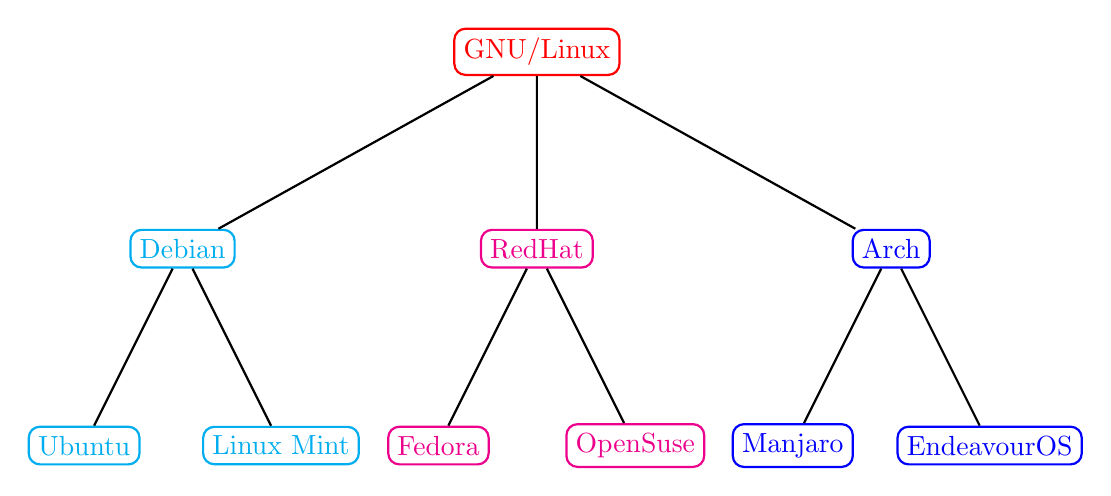
\begin{tikzpicture} [every node/.style = {shape=rectangle, rounded corners, draw,
align=center}]
\path [draw,thick,=]
node (root)[red] {GNU/Linux}
[sibling distance=45mm, level distance=25mm]
child {node [cyan] {Debian}
[sibling distance=25mm, level distance=25mm]
child { node [cyan] {Ubuntu} }
child { node [cyan] {Linux Mint} }
}
child {node [magenta] {RedHat}
[sibling distance=25mm, level distance=25mm]
child { node [magenta] {Fedora} }
child { node [magenta] {OpenSuse} }
}
child {node [blue] {Arch}
[sibling distance=25mm, level distance=25mm]
child { node [blue]{Manjaro} }
child { node [blue]{EndeavourOS} }
};
\end{tikzpicture}
\caption{GNU/Linux Operating System Family}
\end{figure}
\end{document}